% --------------------------------------------------------------
% Abhi's Standard math Preamble.
% --------------------------------------------------------------
 
% Document packages / layout
\documentclass[
  %aspectratio=169,
  pdf,
  10pt,
  xcolor={svgnames},
  %hyperref={colorlinks, citecolor=Cyan, linkcolor=Cyan, urlcolor=Cyan}
]{beamer}
%\usetheme{Copenhagen}
\usetheme{Madrid}
\usecolortheme{beaver}
\usepackage{color}
\setbeamertemplate{navigation symbols}{}%remove navigation symbols

\newcommand\hmmax{0}
\newcommand\bmmax{0}

\usepackage{biblatex}
\addbibresource{citations.bib}

\newcommand\blfootnote[1]{%
  \begingroup
  \renewcommand\thefootnote{}\footnote{\scriptsize #1}%
  \addtocounter{footnote}{-1}%
  \endgroup
}

% Figure Packages
\usepackage{float}
\usepackage{subcaption}

% Math Packages
\usepackage{amsmath, amsthm, amssymb}
\usepackage{commath} %for \norm and \abs
\usepackage{bm}
\usepackage{dsfont}
\usepackage{mathtools}
\usepackage{mathrsfs}
\usepackage{physics}
\usepackage{stmaryrd}
\allowdisplaybreaks

% Quality of Life Packages
\usepackage{enumerate}
\usepackage{siunitx} %\sisetup{inter-unit-product =$\cdot$}
\usepackage{multicol}
\usepackage{todonotes}

\newtheorem*{lemma*}{Lemma}
\newtheorem*{theorem*}{Theorem}
\newtheorem*{definition*}{Definition}

%% general package aliases
\newcommand{\bs}{\boldsymbol}
\def\ds{\displaystyle}
\newcommand{\mb}[1]{\mathbb{#1}}
\newcommand{\mbf}[1]{\mathbf{#1}}
\newcommand{\mc}[1]{\mathcal{#1}}
\newcommand{\mcb}[1]{\boldsymbol{\mathcal{#1}}}
\newcommand{\ms}[1]{\mathscr{#1}}
%% Set aliases
\newcommand{\N}{\mathbb{N}}
\newcommand{\R}{\mathbb{R}}
%% Analysis aliases
\newcommand{\e}{\varepsilon}
\DeclareMathOperator*{\argmin}{\arg\!\min}
\DeclareMathOperator*{\argmax}{\arg\!\max}
\DeclarePairedDelimiterX{\inp}[2]{\langle}{\rangle}{#1, #2}
%% Matrix aliases
\newcommand{\T}{\mathrm{T}}
\renewcommand{\vec}[1]{{\mathchoice
                     {\mbox{\boldmath$\displaystyle{#1}$}}
                     {\mbox{\boldmath$\textstyle{#1}$}}
                     {\mbox{\boldmath$\scriptstyle{#1}$}}
                     {\mbox{\boldmath$\scriptscriptstyle{#1}$}}}}
\newcommand{\mat}[1]{\mathbf{{#1}}}
%% Inverse Problems aliases
\newcommand{\Reg}{\boldsymbol{\mathcal{R}}}
\newcommand{\priormean}{\vec{u}_{0,{\rm pr}}}
\newcommand{\ut}[1]{\ensuremath{\tilde{#1}}}
\newcommand{\ui}[1]{\ensuremath{\hat{#1}}}
\newcommand{\bui}[1]{\ensuremath{\hat{\boldsymbol{#1}}}}
\newcommand{\bu}[1]{\ensuremath{\boldsymbol{#1}}}
\newcommand{\mbu}[1]{\ensuremath{\mathbf{#1}}}
\newcommand{\obs}{\mathbf{u}^{\rm obs}}

\newcommand{\Gnoise}{\mat{\Gamma}_{\rm noise}}

% Creates section subdivider at beginning of each section.
\AtBeginSection[]
{
  \begin{frame}
    \frametitle{Table of Contents}
    \tableofcontents[currentsection]
  \end{frame}
}
 
\title[%
  Eigenvalue Sensitivities for Sensitivity Analysis
]{%
  Computing Eigenvalue Sensitivities for Sensitivity Analysis of the Information
  Gain in Bayesian Linear Inverse Problems
}
\author[Chowdhary, Alexanderian]{%
  Abhijit Chowdhary and Alen Alexanderian
}
\institute[NCSU]{
  Department of Mathematics \\
  North Carolina State University
}
\date[AMGSS 2022]{\today}

\begin{document}

\frame{ \titlepage \scriptsize{ Work done through NSF-DMS-2111044 } }

\begin{frame}
  \begin{figure}
    \centering
    \includegraphics[width=0.85\textwidth]{./resources/Cocos}
  \end{figure}
  \blfootnote{\fullcite{Cocos2006}}
\end{frame}

\begin{frame}
  \begin{figure}
    \centering
    \includegraphics[width=\textwidth]{./resources/subduction_zone}
  \end{figure}
  \blfootnote{\fullcite{Lillie2017}}
\end{frame}

\begin{frame}
  \frametitle{Goals}
  \begin{alertblock}{}
    \begin{center}
      {\large Understand the subduction zone from collected observations.}
    \end{center}
  \end{alertblock}
  \pause
  \begin{alertblock}{}
    \begin{center}
      {\large Do so while quantifying measurement uncertainties.}
    \end{center}
  \end{alertblock}
\end{frame}

\begin{frame}
  \frametitle{Table of Contents}
  \tableofcontents
\end{frame}

%%%%%%%%%%%%%%%%%%%%%%%%%%%%%%%%%%%%%%%%%%%%%%%%%%%%%%%%%%%%%%%%%%%%%%%%%%%%%%%
%%% Seismic Inversion Model Problem
%%%%%%%%%%%%%%%%%%%%%%%%%%%%%%%%%%%%%%%%%%%%%%%%%%%%%%%%%%%%%%%%%%%%%%%%%%%%%%%
\section{Seismic Inversion Model Problem}
\begin{frame}
  \frametitle{Model Assumptions}
  \begin{figure}
    \centering
    \includegraphics[width=0.55\textwidth]{./resources/triangle_paraview}
    %\includegraphics[width=\textwidth]{./resources/subduction_zone}
  \end{figure}
  \begin{itemize}[<+->]
    \item \textbf{Governing PDE} (forward model): Linear elasticity
    \item \textbf{Uncertain parameter}: Displacement on fault plane
    \item \textbf{Inverse Problem}: Given measurements of surface deformation
          $\obs$ reconstruct fault plane displacement.
  \end{itemize}
\end{frame}
\begin{frame}
  \frametitle{Forward Model}
  \begin{equation*}
    -\nabla \cdot \bs \sigma(\bs u) = \bs 0 \text{ in } \Omega,
  \end{equation*}
  where:
  \begin{itemize}
    \item $\vec{\sigma}(\vec{u}) = \mathbb{C} \vec{\varepsilon}(\vec{u})$ with
          \bigskip
          \begin{itemize}
            \item $\mathbb{C}[\vec{\e}] = 2\mu \vec{\e} + \lambda \tr(\vec{\e})
                    \mat{I}$ the fourth-order linear elasticity tensor:
                  \bigskip
            \item $\vec{\e}(\vec{u}) = \frac{1}{2} \left[ \grad \vec{u} + (\grad
                      \vec{u})^\T \right]$ the strain tensor.
                  \bigskip
          \end{itemize}
    \item $\mu$ and $\lambda$ are the L\'{a}me constants.
  \end{itemize}
  \blfootnote{\fullcite{McCormack2018}}
\end{frame}
\begin{frame}
  \frametitle{Forward Model}
  \begin{align*}
    - \grad \left[
      \mu(\grad \vec{u} + (\grad \vec{u})^\T)
      + \lambda \div \vec{u} \mat{I}
      \right]
     & =
    \vec{0} \quad \text{in } \Omega,  \\
    \vec{\sigma}(\vec{u}) \vec{n}
     & =
    \vec{0} \quad \text{on } \Gamma_t \\
    \vec{u} + \beta \vec{\sigma}(\vec{u}) \vec{n}
     & =
    \vec{h} \quad \text{on } \Gamma_s \\
    \vec{u} \vdot \vec{n}
     & =
    0 \quad \text{on } \Gamma_b       \\
    \delta \mat{T}(\vec{\sigma}(\vec{u})\vec{n}) + \mat{T}\vec{u}
     & =
    \vec{m} \quad \text{on } \Gamma_b
  \end{align*}
  \begin{itemize}[<+->]
    \item $\mat{T}$ is the tangential operator $\mat{T} \vec{u} = (\mat{I}
            - \vec{n} \otimes \vec{n}) \vec{u} = \vec{u} - (\vec{n}^\T \vec{u})
            \vec{n}$.
    \item $\vec{m}$ is the displacement
          on the fault plane that is being inverted for.
  \end{itemize}
\end{frame}

%\begin{frame}
%  \frametitle{Mesh}
%  \begin{figure}
%    \centering
%    \includegraphics[width=0.5\textwidth]{./resources/mesh_side}
%  \end{figure}
%\end{frame}
\begin{frame}
  \frametitle{Mesh}
  \begin{figure}
    \centering
    \includegraphics[width=0.49\textwidth]{./resources/mesh_bot}
    \includegraphics[width=0.49\textwidth]{./resources/mesh_top}
  \end{figure}
\end{frame}

\begin{frame}
  \frametitle{Forward Solution}
  \begin{figure}
    \centering
    \includegraphics[width=0.49\textwidth]{./resources/fwd_bot}
    \includegraphics[width=0.49\textwidth]{./resources/fwd_top}
  \end{figure}
\end{frame}
\begin{frame}
  \frametitle{Forward Solution}
  \begin{figure}
    \centering
    \includegraphics[width=0.49\textwidth]{./resources/fwd_bot_log}
    \includegraphics[width=0.49\textwidth]{./resources/fwd_top_log}
  \end{figure}
\end{frame}

%%%%%%%%%%%%%%%%%%%%%%%%%%%%%%%%%%%%%%%%%%%%%%%%%%%%%%%%%%%%%%%%%%%%%%%%%%%%%%%%
%%% Bayesian Inversion Setting
%%%%%%%%%%%%%%%%%%%%%%%%%%%%%%%%%%%%%%%%%%%%%%%%%%%%%%%%%%%%%%%%%%%%%%%%%%%%%%%%
\section{Infinite-Dimensional Inverse Problem Setting}
\begin{frame}
  \frametitle{The Deterministic Inverse Problem}
  To reconstruct the fault displacement we construct the PDE-constrained
  optimization problem:
  \[
    \mc{J}(\vec{m})
    = \frac{1}{2} \| \mcb{B}\vec{u}(\vec{m}) - \obs \|^2
    + \frac{1}{2} \| \mc{R}\vec{m} \|^2
  \]
  where $\vec{u}$ is given by the solution of the linear elasticity equation.
  \begin{itemize}
    \item $\vec{u}(\vec{m})$ is given by the forward model.
    \item $\mcb{B}: (L^2(\Omega))^3 \to \R^N$ is an observation operator.
    \item $\obs \in \R^N$ where $N$ is the number of data points.
    \item $\mc{R}$ is some regularization operator.
  \end{itemize}
  \pause
  If we let $\mcb{S}$ be the forward model operator, i.e. $\vec{u} = \mcb{S}
    \vec{m}$, and let\footnote{%
    In literature, called the {\em parameter-to-observable operator}.
  } $\mcb{F} = \mcb{B} \mcb{S}$, then:
  \[
    \mc{J}(\vec{m})
    = \frac{1}{2} \| \mcb{F}\vec{m} - \obs \|^2
    + \frac{1}{2} \| \mc{R}\vec{m} \|^2
  \]
\end{frame}

\begin{frame}
  \frametitle{Bayesian Inversion in Infinite Dimensions}
  \begin{theorem}[Bayes Theorem in Infinite Dimensions]
    \[
      \dv{\mu^{\obs}_{\rm post}}{\mu_{\rm pr}}
      \propto
      \pi_{\rm like}(\obs | \vec{m})
    \]
  \end{theorem}
  \begin{itemize}
    \item Gaussian Prior $\vec{m} \sim \mc{N}(\vec{m}_{\rm pr}, \mcb{C}_0)$.
    \item Additive Gaussian noise
          \[
            \obs = \mcb{F} \vec{m} + \vb*{\eta},
            \quad \vb*{\eta} \sim \mc{N}(\vb{0}, \mat{\Gamma}_{\rm noise})
          \]
    \item Gaussian posterior:
          \[
            \mu^{\obs}_{\rm post}
            =
            \mc{N}(\vec{m}_{\rm post} , \mcb{C}_{\rm post})
          \]
          where:
          \begin{align*}
            \vec{m}_{\rm post}
             & =
            \mcb{C}_{\rm post}
            \left(
            \mcb{F}^* \vb{\Gamma}_{\rm noise}^{-1} \obs
            + \mcb{C}_{\rm pr}^{-1} \vec{m}_{\rm pr}
            \right)      \\
            \mcb{C}_{\rm post}
             & =
            \left(
            \mcb{F}^* \vb{\Gamma}_{\rm noise}^{-1} \mcb{F}
            + \mcb{C}_{\rm pr}^{-1}
            \right)^{-1} \\
          \end{align*}
  \end{itemize} \vspace{-1em}
  %Corresponds to
  %\(
  %  \mc{J}(\vec{m})
  %  = \frac{1}{2} \| \mc{F}\vec{m} - \obs \|_{\vb{\Gamma}_{\rm noise}^{-1}}^2
  %  + \frac{1}{2} \| \mc{C}^{-1/2}(\vec{m}-\vec{m}_{\rm pr}) \|^2
  %\).
\end{frame}

\begin{frame}
  \frametitle{MAP Estimation vs. True Parameter}
  \begin{figure}
    \centering
    \includegraphics[width=0.48\textwidth]{./resources/m_true}
    \includegraphics[width=0.48\textwidth]{./resources/map_m}
  \end{figure}
\end{frame}
\begin{frame}
  \frametitle{Prior Samples}
  \begin{figure}
    \centering
    \includegraphics[width=0.48\textwidth]{./resources/prior_sample_1}
    \includegraphics[width=0.48\textwidth]{./resources/prior_sample_2}
    %\includegraphics[width=0.30\textwidth]{./resources/prior_sample_3}
  \end{figure}
\end{frame}
\begin{frame}
  \frametitle{Posterior Samples}
  \begin{figure}
    \centering
    \includegraphics[width=0.48\textwidth]{./resources/post_sample_1}
    \includegraphics[width=0.48\textwidth]{./resources/post_sample_2}
    %\includegraphics[width=0.30\textwidth]{./resources/post_sample_3}
  \end{figure}
\end{frame}

%%%%%%%%%%%%%%%%%%%%%%%%%%%%%%%%%%%%%%%%%%%%%%%%%%%%%%%%%%%%%%%%%%%%%%%%%%%%%%%
%%% Information Gain as an Objective for UQ
%%%%%%%%%%%%%%%%%%%%%%%%%%%%%%%%%%%%%%%%%%%%%%%%%%%%%%%%%%%%%%%%%%%%%%%%%%%%%%%
\section{Measuring Posterior Uncertainty}
\begin{frame}
  \begin{figure}
    \centering
    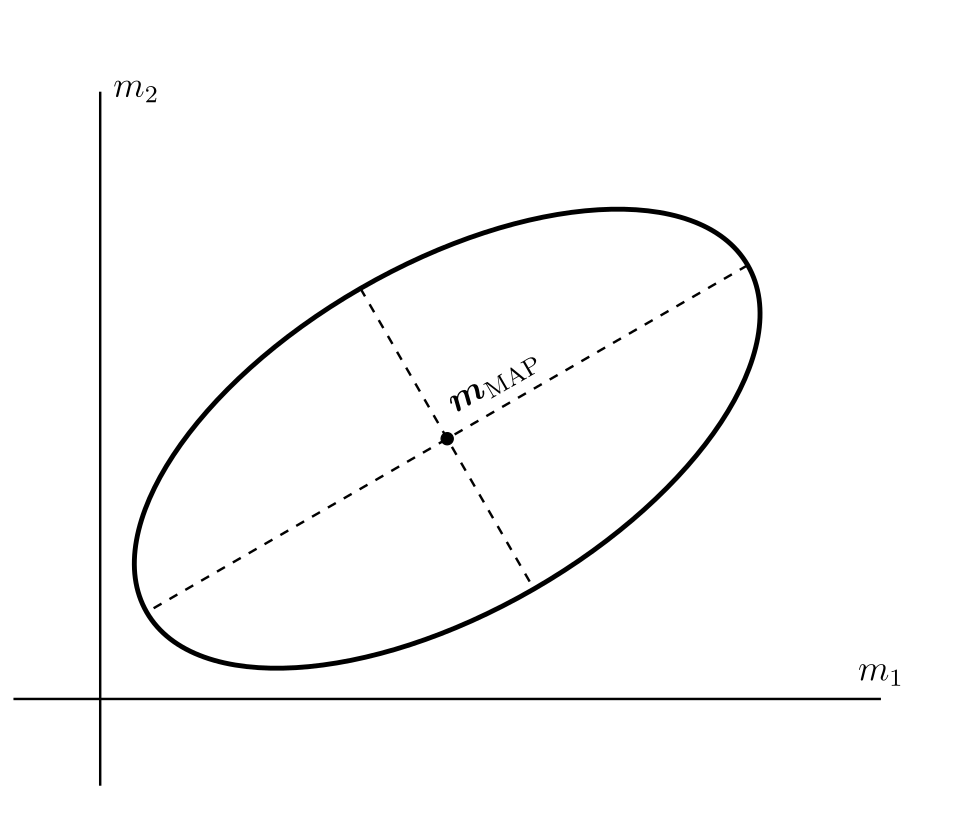
\includegraphics[width=.65\textwidth]{./resources/bivariate}
    \caption{
      The confidence region corresponding to a linear inverse problem with a
      bivariate Gaussian posterior.
    }
  \end{figure}
\end{frame}

\begin{frame}
  \frametitle{Data-Misfit Hessian}
  \begin{definition}[Data-Misfit Hessian]
    The action of the data-misfit Hessian is given by:
    expressed as:
    \begin{equation*}
      \mcb{H} = \mcb{F}^* \mat{\Gamma}_{\rm noise}^{-1} \mcb{F}
    \end{equation*}
  \end{definition}
  \pause
  \begin{definition}[Prior-Preconditioned Data-Misfit Hessian]
    \begin{equation*}
      \tilde{\mcb{H}}
      = \mcb{C}_{\rm prior}^{1/2} \mcb{H} \mcb{C}_{\rm prior}^{1/2}
    \end{equation*}
    Let $\{(\lambda_i, \psi_i)\}_{i=1}^k$ be the dominant eigenpairs of
    $\tilde{\mcb{H}}$, then:
    \[
      \tilde{\mcb{H}} v \approx \sum_{i=1}^k \lambda_i \inp{\psi_i}{v} \psi_i
    \]
    is a low rank approximation of $\tilde{\mcb{H}}$.
  \end{definition}
\end{frame}

\begin{frame}
  \frametitle{A Measure of Posterior Uncertainty}
  \begin{definition}[Kullback-Leibler Divergence]
    The KL-Divergence from the posterior to the prior quantifies the information
    gain and in the context of Bayesian linear inverse problems has the form:
    \begin{align*}
      \Phi_{\rm KL}
       & =
      \frac{1}{2}\left[
      \log\det(\tilde{\mcb{H}} + \mcb{I})
      - {\rm trace}\left(
      \tilde{\mcb{H}}(\mcb{I} + \tilde{\mcb{H}})^{-1}
      \right)
      + \norm{
        \vec{m}_{\rm MAP} - \vec{m}_{\rm pr}
      }_{\mat{\Gamma}_{\rm noise}^{-1}}^2
      \right]    \\
       & \approx
      \sum_{j=1}^k
      \frac{1}{2}\left[
      \log(\lambda_j + 1)
      - \frac{\lambda_j}{1+\lambda_j}
      + {\norm{
        \vec{m}_{\rm MAP} - \vec{m}_{\rm pr}
      }_{\mat{\Gamma}_{\rm noise}^{-1}}^2}
      \right]
    \end{align*}
  \end{definition}
  \pause
  To assess the sensitivity of a Bayesian inverse problem with respect to
  modeling uncertaintities, we compute partial derivative of $\Phi_{\rm KL}$
  with respect to said model parameters.
  \pause
  \begin{alertblock}{}
    \begin{center}
      {\bf Q:} How do we differentiate this expression?
    \end{center}
  \end{alertblock}
\end{frame}
\begin{frame}
  \begin{alertblock}{}
    \begin{center}
      {\bf Q:} How do we differentiate this expression?
    \end{center}
  \end{alertblock}
  \[
    \Phi_{\rm KL}
    = \approx
    \sum_{j=1}^k
    \frac{1}{2}\left[
      \underbrace{
        \log(\lambda_j + 1)
        - \frac{\lambda_j}{1+\lambda_j}
      }_{\text{Eigenvalue Sensitivities}}
      + \underbrace{
        \norm{
          \vec{m}_{\rm MAP} - \vec{m}_{\rm pr}
        }_{\mat{\Gamma}_{\rm noise}^{-1}}^2
      }_{\text{HDSA}}
      \right]
  \]
  \blfootnote{\fullcite{Sunseri2020}}
\end{frame}

%%%%%%%%%%%%%%%%%%%%%%%%%%%%%%%%%%%%%%%%%%%%%%%%%%%%%%%%%%%%%%%%%%%%%%%%%%%%%%%
%%% Eigenvalue Sensitivities: Finite Dimensional Example
%%%%%%%%%%%%%%%%%%%%%%%%%%%%%%%%%%%%%%%%%%%%%%%%%%%%%%%%%%%%%%%%%%%%%%%%%%%%%%%
\section{Eigenvalue Sensitivity: Finite Dimensional Example}
\begin{frame}
  \frametitle{Simple Finite Dimensional Example}
  Consider an implicitly defined matrix $\mat{H}$ whose action is defined by:
  \begin{subequations}\label{equ:Hdef}
    \begin{alignat}{2}
       & \mat{H} \mbf{v} \coloneqq  \mat{C}^\T \mbf{p}                    \\
       & \text{where}\notag                                               \\
       & \mat{A}(\theta) \mbf{u} + \mat{C} \mbf{v} = \mbf{0}              \\
       & \mat{A}(\theta)^\T \mbf{p} + \mat{B}^\T\mat{B} \mbf{u} = \mbf{0}
    \end{alignat}
  \end{subequations}
  Furthermore, consider $\tilde{\mat{H}} = \mat{\Gamma}^{1/2} \mat{H}
    \mat{\Gamma}^{1/2}$ with $\mat{\Gamma}$ symmetric positive definite.
  \pause
  \begin{alertblock}{}
    To illustrate eigenvalue sensitivity analysis, we consider sensitivity of
    the largest eigenvalue of $\tilde{\mat{H}}$ with respect to $\theta$.
  \end{alertblock}
  \pause
  \begin{alertblock}{Note:}
    Let $(\lambda, \mbf{w})$ be the dominant eigenpair of $\tilde{\mat{H}}$,
    then $\mat{H} \mbf{v} = \lambda \mat{\Gamma}^{-1} \mbf{v}$ with $\mbf{v} =
      \mat{\Gamma}^{1/2} \mbf{w}$.
  \end{alertblock}
\end{frame}
\begin{frame}
  \frametitle{Derivation}
  We can define $\lambda$ as a function of uncertain model parameters implicitly:
  \begin{align*}
     &
    \lambda(\theta)
    = \mbf{v}^\T \mat{C}^\T \mbf{p}        \\
     & \text{where}\notag                  \\
     &
    \mat{A}(\theta)\mbf{u}
    + \mat{C} \mbf{v} = \mbf{0}            \\
     &
    \mat{A}({\theta})^\top \mbf{p}
    + \mat{B}^\T \mat{B} \mbf{u} = \mbf{0} \\
     &
    \mbf{v}^\T \mat{\Gamma}^{-1}\mbf{v}
    - 1 = 0
  \end{align*}
  \pause
  \begin{definition}
    To facilitate derivative computation, we consider the "meta-Lagrangian":
    \begin{equation*}
      \mc{L}
      = \inp{\mbf{v}}{\mat{C}^\T \mbf{p}}
      + \inp{\mbf{p}^*}{\mat{A}(\theta)\mbf{u} + \mat{C} \mbf{v}}
      + \inp{\mbf{u}^*}{
        \mat{A}(\theta)^\T \mbf{p} - \mat{B}^\T \mat{B} \mbf{u}
      }
      + \lambda^* \left( 1-\mbf{v}^\top \mat{\Gamma}^{-1} \mbf{v} \right)
    \end{equation*}
  \end{definition}
\end{frame}

\begin{frame}
  \frametitle{Solving for Lagrange Multipliers}
  \begin{block}{}
    \begin{equation*}
      \mc{L}
      = \inp{\mbf{v}}{\mat{C}^\T \mbf{p}}
      + \inp{\mbf{p}^*}{\mat{A}(\theta)\mbf{u} + \mat{C} \mbf{v}}
      + \inp{\mbf{u}^*}{
        \mat{A}(\theta)^\T \mbf{p} - \mat{B}^\T \mat{B} \mbf{u}
      }
      + \lambda^* \left( 1-\mbf{v}^\top \mat{\Gamma}^{-1} \mbf{v} \right)
    \end{equation*}
  \end{block}
  \begin{align*}
    \mc{L}_\mbf{u}
     & = \mat{A}^\top \mbf{p}^* + \mat{B}^\top\mat{B} \mbf{u}^* = 0       \\
    \mc{L}_\mbf{p}
     & = \mat{A} \mbf{u}^* + \mat{C} \mbf{v} = 0                          \\
    \mc{L}_\mbf{v}
     & = 2\mat{C}^\top \mbf{p} - 2\lambda^* \mat{\Gamma}^{-1} \mbf{v} = 0
  \end{align*}
\end{frame}
\begin{frame}
  \frametitle{Solving for Lagrange Multipliers}
  \begin{block}{}
    \begin{equation*}
      \mc{L}
      = \inp{\mbf{v}}{\mat{C}^\T \mbf{p}}
      + \inp{\mbf{p}^*}{\mat{A}(\theta)\mbf{u} + \mat{C} \mbf{v}}
      + \inp{\mbf{u}^*}{
        \mat{A}(\theta)^\T \mbf{p} - \mat{B}^\T \mat{B} \mbf{u}
      }
      + \lambda^* \left( 1-\mbf{v}^\top \mat{\Gamma}^{-1} \mbf{v} \right)
    \end{equation*}
  \end{block}
  \begin{minipage}{.5\linewidth}
    \begin{align*}
      \mc{L}_\mbf{u}
       & = \mat{A}^\top \mbf{p}^* + \mat{B}^\top\mat{B} \mbf{u}^* = 0       \\
      \mc{L}_\mbf{p}
       & = \mat{A} \mbf{u}^* + \mat{C} \mbf{v} = 0                          \\
      \mc{L}_\mbf{v}
       & = 2\mat{C}^\top \mbf{p} - 2\lambda^* \mat{\Gamma}^{-1} \mbf{v} = 0
    \end{align*}
  \end{minipage}%
  \begin{minipage}{.5\linewidth}
    \begin{align*}
       &
      \lambda(\theta)
      = \mbf{v}^\T \mat{C}^\T \mbf{p}        \\
       & \text{where}\notag                  \\
       &
      \mat{A}(\theta)\mbf{u}
      + \mat{C} \mbf{v} = \mbf{0}            \\
       &
      \mat{A}({\theta})^\top \mbf{p}
      + \mat{B}^\T \mat{B} \mbf{u} = \mbf{0} \\
       &
      \mbf{v}^\T \mat{\Gamma}^{-1}\mbf{v}
      - 1 = 0
    \end{align*}
  \end{minipage}
  That is, $\mbf{u}^* = \mbf{u}$ and $\mbf{p}^* = \mbf{p}$. \pause Regarding
  $\lambda^*$:
  \[
    0 =
    2\mbf{p}^\T \mat{C}^\top \mbf{p}
    - 2\lambda^* \mbf{p}^\T \mat{\Gamma}^{-1} \mbf{v}
    = 2 \lambda - 2 \lambda^*
    \implies \lambda = \lambda^*
  \]
\end{frame}

\begin{frame}
  \frametitle{Eigenvalue Sensitivity}
  \begin{block}{}
    \begin{equation*}
      \mc{L}
      = \inp{\mbf{v}}{\mat{C}^\T \mbf{p}}
      + \inp{\mbf{p}^*}{\mat{A}(\theta)\mbf{u} + \mat{C} \mbf{v}}
      + \inp{\mbf{u}^*}{
        \mat{A}(\theta)^\T \mbf{p} - \mat{B}^\T \mat{B} \mbf{u}
      }
      + \lambda^* \left( 1-\mbf{v}^\top \mat{\Gamma}^{-1} \mbf{v} \right)
    \end{equation*}
  \end{block}
  Finally, $\mc{L}_{\theta_j}$ simplifies to
  \begin{equation*}
    \mc{L}_{\theta_j} =
    \inp{\mbf{p}^*}{[\partial_j\mat{A}] \mbf{u}}
    + \inp{\mbf{u}^*}{[\partial_j\mat{A}]^\top \mbf{p}}
    =
    2\inp{\mbf p}{[\partial_j\mat{A}] \mbf{u}}
  \end{equation*}
  \pause
  Therefore, to compute the sensitivity of $\lambda$ with respect to $\theta_j$,
  we have the following algorithm:
  \begin{itemize}[<+->]
    \item solve the eigenproblem for eigenvector $\mbf{v}$
    \item solve $\mat{A} \mbf{u} + \mat{C} \mbf{v} = \mbf{0}$ for $\mbf{u}$
    \item solve $\mat{A}^\T \mbf{p} + \mat{B}^\T\mat{B}\mbf{u} = \mbf{0}$ for
          $\mbf{p}$
    \item evaluate eigenvalue sensitivities \(
          \partial_j \lambda(\mbf\theta)
          = 2\inp{\mbf p}{[\partial_j\mat{A}] \mbf{u}},
          \quad j \in \{1, \ldots, N\}
          \)
  \end{itemize}
\end{frame}
\begin{frame}
  \frametitle{Simple Numerical Example}
  \[
    \mat{A} = \begin{bmatrix}
      -20 (1 + a_2\theta_2) & 3(1 + a_3\theta_3)    & 0                     \\
      1 + a_1 \theta_1      & -20 (1 + a_2\theta_2) & 3(1 + a_3\theta_3)    \\
      0                     & 1 + a_1 \theta_1      & -20 (1 + a_2\theta_2)
    \end{bmatrix}, \quad \mbf{a} = \begin{bmatrix}0.08 & 0.06 & 0.09\end{bmatrix}^\top.
  \]
  Also, the remaining matrices for the present example are as follows:
  \[
    \mat{B} = \begin{bmatrix} 1 & -1 & 1 \\  -1 & 1 & 1 \end{bmatrix} \quad
    \mat{C} = \begin{bmatrix} 1 & 2 \\ 3 & 4 \\  5 & 6\end{bmatrix}, \quad
    \mat{\Gamma} = \begin{bmatrix} 3 & 0 & 0\\ 0 & 2 & 0 \\ 0 & 0 & 1\end{bmatrix}.
  \]
  In this case, the matrix $\mat{H}$ is a $2 \times 2$ matrix.
\end{frame}
\begin{frame}
  \begin{figure}
    \centering
    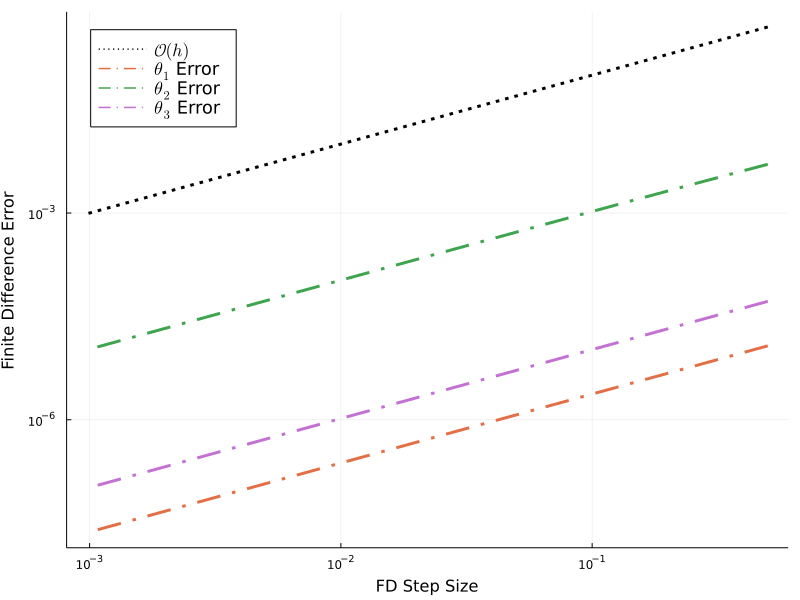
\includegraphics[width=.8\textwidth]{./resources/findim_fd_err.png}
    \caption{Forward finite difference error vs. exact}
  \end{figure}
\end{frame}

%%%%%%%%%%%%%%%%%%%%%%%%%%%%%%%%%%%%%%%%%%%%%%%%%%%%%%%%%%%%%%%%%%%%%%%%%%%%%%%
%%% Eigenvalue Sensitivities: Infinite Dimensional Example
%%%%%%%%%%%%%%%%%%%%%%%%%%%%%%%%%%%%%%%%%%%%%%%%%%%%%%%%%%%%%%%%%%%%%%%%%%%%%%%
\section{Eigenvalue Sensitivity: Infinite Dimensional Example}
\begin{frame}
  \frametitle{Simple Infinite Dimensional Example}
  For a domain $\Omega \subset \R^n$ with boundary $\partial \Omega$, consider the
  elliptic PDE:
  \begin{align*}
    -\laplacian u + c u & = f, \quad \text{in } \Omega         \\
    \grad u \vdot n     & = g, \quad \text{in } \partial\Omega
  \end{align*}
  \begin{alertblock}{Bayesian Linear Inverse Problem}
    Using measurements of $u$ on $\Omega$, we seek to estimate $f$.
  \end{alertblock}
  \pause
  \begin{alertblock}{Goal:}
    Study the sensitivity of the largest eigenvalue of the data-misfit Hessian
    for the inversion with respect to constant $c$.
  \end{alertblock}
  \pause
  \begin{align*}
     & \mc{L}(u,p,f)
    = \frac{1}{2} \norm{\mc{B}u(f) - \obs}_{\Gnoise^{-1}}^2
    + \frac{1}{2} \norm{f - f_{\rm pr}}_{\mc{C}_0^{-1}}^2 \\
     & \quad
    \int_\Omega \grad u \vdot \grad p \dd{x}
    + c \int_\Omega up \dd{x}
    - \int_\Omega fp \dd{x}
    - \int_{\partial\Omega} gp \dd{s}
  \end{align*}
\end{frame}

\begin{frame}
  \frametitle{The adjoint based expression the data-misfit Hessian action}
  Taking variations in $u,p$ and $f$ twice, we find the data-misfit Hessian:
  \[
    \mc{L}^H_f(\tilde{f})
    =
    \underbrace{
      - \int_\Omega \tilde{f} \hat{p} \dd{x}
    }_{\mc{H}(f)(\hat{f},\tilde{f})}
    + \inp{\tilde{f}}{\hat{f}}_{\mc{C}_0^{-1}}
  \]
  which, to evaluate in direction $\hat{f}$, we need to solve the incremental
  system:
  \begin{align*}
    \mc{L}^H_v(\tilde{p})
     & =
    \int_\Omega \grad \hat{u} \vdot \grad \tilde{p} \dd{x}
    + c\int_\Omega \hat{u} \tilde{p} \dd{x}
    - \int_\Omega \hat{f} \tilde{p} \dd{x}
     & = 0, \quad \forall \tilde{p} \in V \\
    \mc{L}^H_u(\tilde{u})
     & =
    \int_\Omega \grad \tilde{u} \vdot \grad \hat{p} \dd{x}
    + c \int_\Omega \tilde{u} \hat{p} \dd{x}
    + \inp{\mc{B} \tilde{u}}{\mc{B}\hat{u}}_{\Gnoise^{-1}}
     & = 0, \quad \forall \tilde{u} \in V
  \end{align*}
\end{frame}

\begin{frame}
  \frametitle{Eigenproblem Constraint}
  \begin{align*}
    \int_\Omega \grad \hat{u} \vdot \grad \tilde{p} \dd{x}
    + c\int_\Omega \hat{u} \tilde{p} \dd{x}
    - \int_\Omega \psi \tilde{p} \dd{x}
     & = 0,
     & \quad \forall \tilde{p} \in V \\
    \int_\Omega \grad \tilde{u} \vdot \grad \hat{p} \dd{x}
    + c \int_\Omega \tilde{u} \hat{p} \dd{x}
    + \inp{\mc{B} \tilde{u}}{\mc{B}\hat{u}}_{\Gnoise^{-1}}
     & = 0,
     & \quad \forall \tilde{u} \in V \\
    -\int_\Omega \phi \hat{p} \dd{x}
     & =
    \lambda \inp{\phi}{\psi}_{\mc{C}_0^{-1}},
     & \quad \forall \phi \in V      \\
    1 - \inp{\psi}{\psi}_{\mc{C}_0^{-1}}
     & = 0
     &
  \end{align*}
  \pause
  \begin{align*}
     & ~ \mc{L}^E(\hat{u},\hat{p},\psi,\hat{u}^*,\hat{p}^*,\lambda^*)
    = \left[
      -\int_\Omega \psi \hat{p} \dd{x}
      \right]
    + \lambda^* \left[
    1 - \inp{\psi}{\psi}_{\mc{C}_0^{-1}}
    \right]                                                           \\
     & ~
    + \left[
      \int_\Omega \grad \hat{u} \vdot \grad \hat{p}^* \dd{x}
      + c\int_\Omega \hat{u} \hat{p}^* \dd{x}
      - \int_\Omega \psi \hat{p}^* \dd{x}
    \right]                                                           \\
     & ~
    + \left[
      \int_\Omega \grad \hat{u}^* \vdot \grad \hat{p} \dd{x}
      + c \int_\Omega \hat{u}^* \hat{p} \dd{x}
      + \inp{\mc{B} \hat{u}^*}{\mc{B}\hat{u}}_{\Gnoise^{-1}}
      \right]
  \end{align*}

\end{frame}

\begin{frame}
  \frametitle{Solving for Lagrange Multipliers}
  \begin{align*}
    \mc{L}^E_{\hat{p}}(\tilde{p})
     & =
    \int_\Omega \grad \hat{u}^* \vdot \grad \tilde{p} \dd{x}
    + c \int_\Omega \hat{u}^* \tilde{p} \dd{x}
    -\int_\Omega \psi \tilde{p} \dd{x}
     & = 0, \forall \tilde{p} \in V    \\
    \mc{L}^E_{\hat{u}}(\tilde{u})
     & =
    \int_\Omega \grad \tilde{u} \vdot \grad \hat{p}^* \dd{x}
    + c\int_\Omega \tilde{u} \hat{p}^* \dd{x}
    + \inp{\mc{B} \hat{u}^*}{\mc{B}\tilde{u}}_{\Gnoise^{-1}}
     & = 0, \forall \tilde{u} \in V    \\
    \mc{L}^E_{\psi}(\tilde{\psi})
     & =
    -2 \int_\Omega \tilde{\psi} \hat{p} \dd{x}
    -2 \lambda^* \inp{\psi}{\tilde{\psi}}_{\mc{C}_0^{-1}}
     & = 0, \forall \tilde{\psi} \in V
  \end{align*}
\end{frame}
\begin{frame}
  \frametitle{Solving for Lagrange Multipliers: Relating it Back}
  \begin{align*}
    \mc{L}^E_{\hat{p}}(\tilde{p})
     & =
    \underbrace{
      \int_\Omega \grad \hat{u}^* \vdot \grad \tilde{p} \dd{x}
      + c \int_\Omega \hat{u}^* \tilde{p} \dd{x}
    }_{\tilde{\mbf{p}}^\T \mat{A} \hat{\mbf{u}}^*}
    \underbrace{
      -\int_\Omega \psi \tilde{p} \dd{x}
    }_{\tilde{\mbf{p}}^\T \mat{C} \mbf{\psi}}
     & = 0, \forall \tilde{p} \in V    \\
    \mc{L}^E_{\hat{u}}(\tilde{u})
     & =
    \underbrace{
      \int_\Omega \grad \tilde{u} \vdot \grad \hat{p}^* \dd{x}
      + c\int_\Omega \tilde{u} \hat{p}^* \dd{x}
    }_{\tilde{\mbf{u}}^\T \mat{A}^\T \hat{\mbf{p}}^*}
    + \inp{\mc{B} \hat{u}^*}{\mc{B}\tilde{u}}_{\Gnoise^{-1}}
     & = 0, \forall \tilde{u} \in V    \\
    \mc{L}^E_{\psi}(\tilde{\psi})
     & =
    -2 \int_\Omega \tilde{\psi} \hat{p} \dd{x}
    -2 \lambda^* \inp{\psi}{\tilde{\psi}}_{\mc{C}_0^{-1}}
     & = 0, \forall \tilde{\psi} \in V
  \end{align*}
  Like in the finite dimensional example, we find $\hat{u}^* = \hat{u},
    \hat{p}^* = \hat{p}$ and $\lambda^* = \lambda$. Hence:
  \[
    \mc{L}^E_c
    =
    \int_\Omega \hat{u} \hat{p}^* \dd{x}
    + \int_\Omega \hat{u}^* \hat{p} \dd{x}
    =
    2\int_\Omega \hat{u} \hat{p} \dd{x}
  \]
\end{frame}
\begin{frame}
  \frametitle{Forward finite difference error vs. exact}
  \begin{figure}
    \centering
    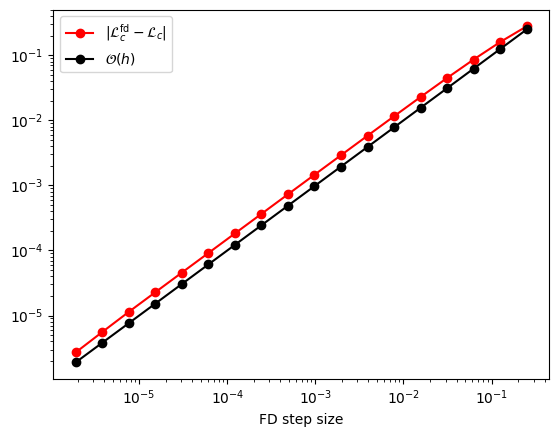
\includegraphics[width=.65\textwidth]{./resources/infdim_fd_err.png}
  \end{figure}
\end{frame}

%%%%%%%%%%%%%%%%%%%%%%%%%%%%%%%%%%%%%%%%%%%%%%%%%%%%%%%%%%%%%%%%%%%%%%%%%%%%%%%
%%% Conclusion and Future Work
%%%%%%%%%%%%%%%%%%%%%%%%%%%%%%%%%%%%%%%%%%%%%%%%%%%%%%%%%%%%%%%%%%%%%%%%%%%%%%%
\begin{frame}
  \frametitle{Conclusion}
  In summary,
  \begin{itemize}
    \item Eigenvalue Sensitivities is a scalable and exact method of leveraging
          existing structures to compute derivatives of eigenvalue based expressions.
    \item Avoids difficulties in finite-difference methods resolving and solves
          half the puzzle of using the information gain as a sensitivity objective.
  \end{itemize}
  \pause
  \begin{block}{Future Work}
    Wrap up sensitivity analysis of the Costa-Rica problem via the
    KL-Divergence.
    \begin{itemize}
      \item Complete HDSA portion of KL Divergence sensitivities
      \item Interpret Sensitivities in terms of real-world model
    \end{itemize}
  \end{block}
\end{frame}

\end{document}